\chapter{Introduction}

\begin{figure}
\centering
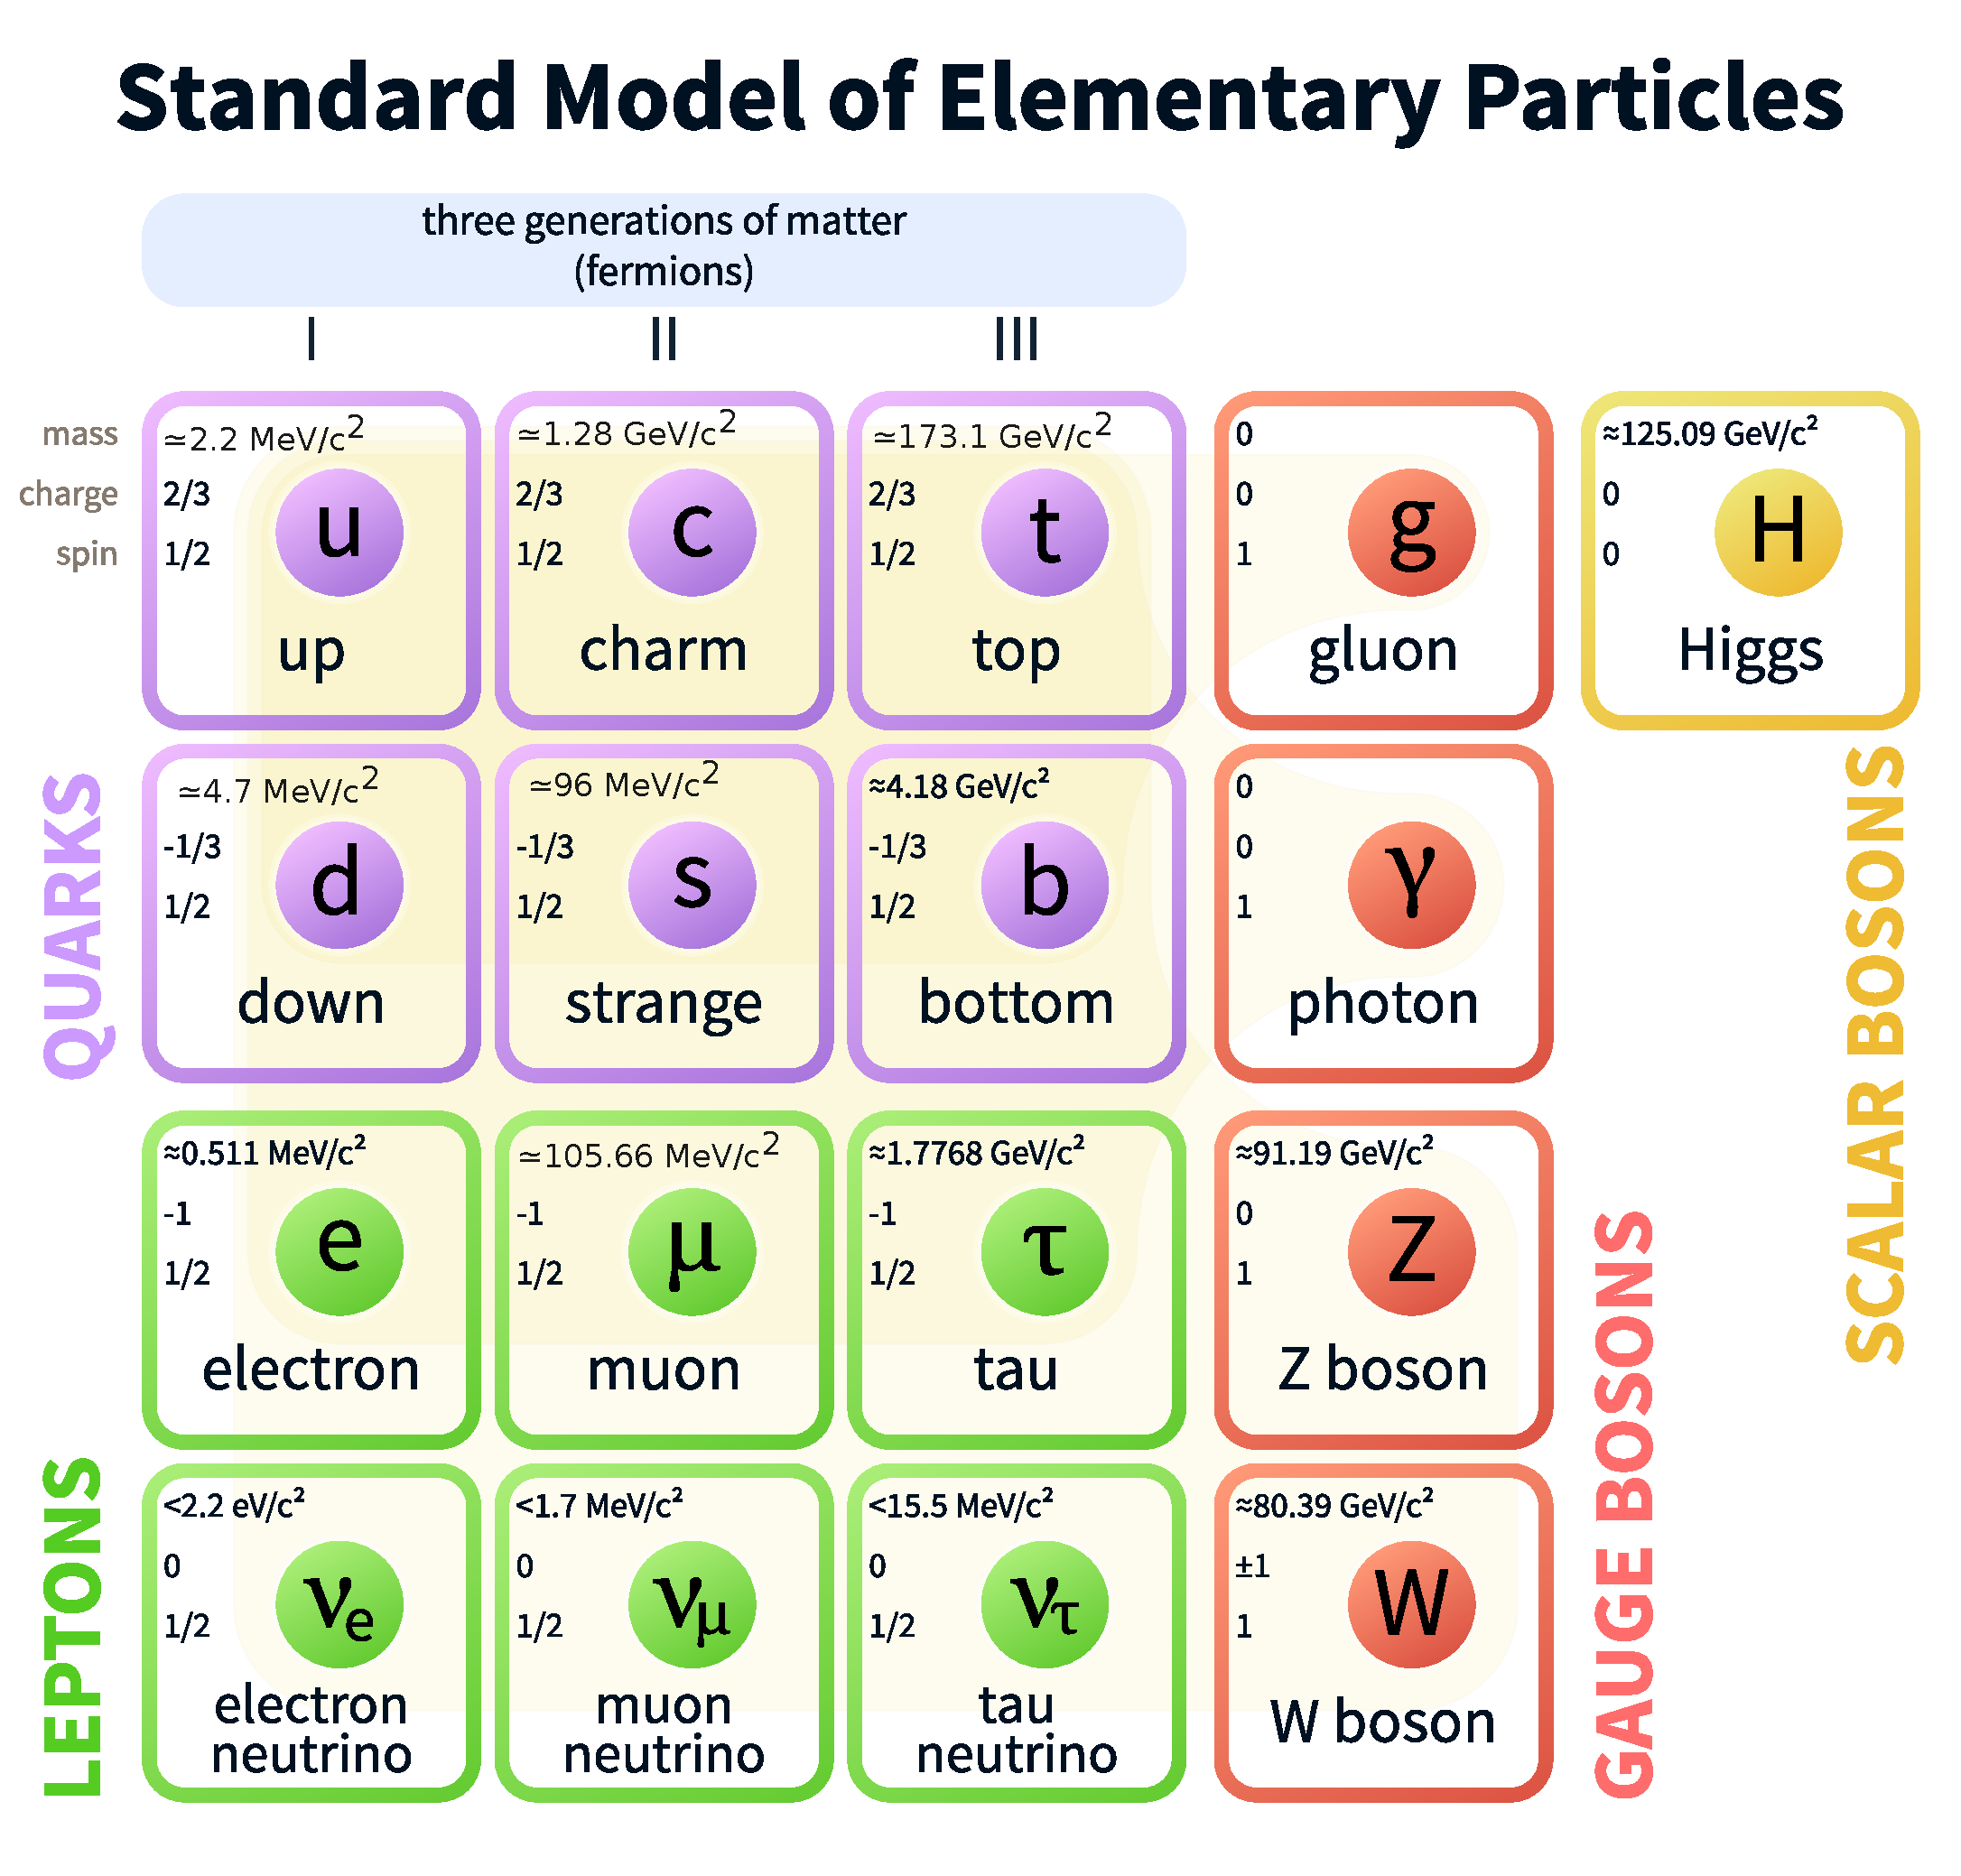
\includegraphics[width=0.6\textwidth]{figs/StandardModelofElementaryParticles.pdf}
\caption{The Standard Model of Particle Physics.}
\label{fig:sm}
\end{figure}

The thesis is outlined as follows: A description of the Standard Model (SM) of particle physics is presented in Chapter~\ref{chap:sm}. A description of the Minimal Supersymmetric Standard Model (MSSM) is presented in Chapter~\ref{chap:mssm}. A description of the Large Hadron Collider (LHC), the facility which acts as our source of high-energy proton-proton collisions, is presented in Chapter~\ref{chap:lhc}. A description of the CMS particle detector, situated to detect the fragments of the proton collisions, is presented in Chapter~\ref{chap:detector}. A description of how the data from the detector are reconstructed and identified as physical particles is presented in Chapter~\ref{chap:eventreco}. The focus of the thesis, a description of the how the physics data can be used to search for evidence of new particles such as those predicted by SUSY, is presented in Chapter~\ref{chap:analysis}. The conclusions are presented in Chapter~\ref{chap:conclusions}. Appendix~\ref{chap:reinterpretation} provides resources for additional physics interpretations of our results presented here. Appendix~\ref{chap:bbsf} presents the calculation of data-mc scale factors for $b\bar{b}$-tagging W boson jets.
